% !TeX root = ../tesis.tex
%%%%%%%%%%%%%%%%%%%%%%%%%%%%%%%%%%%%%%%%%%%%%%%%%%%%%%%%%%%%%%%%%%%
% ANEXO E — Cartografía de Presentación: Transport-gis-zmvm-mjg
%%%%%%%%%%%%%%%%%%%%%%%%%%%%%%%%%%%%%%%%%%%%%%%%%%%%%%%%%%%%%%%%%%%

Este anexo reúne las versiones cartográficas de alta resolución producidas por el sistema \textbf{Transport-gis-zmvm-mjg},
generadas con QGIS~3.x a partir de las plantillas institucionales de la \textsc{unam}. Los mapas utilizan la proyección
\textsc{epsg}:32614 (UTM zona~14N) y tienen como fuente base los \textit{feeds} \gtfs{} de la \textsc{semovi} (2024) y la cartografía
del \textsc{inegi} (2023). Versiones reducidas de estos mapas se encuentran en los capítulos~\ref{ch:Capas-codigo}
y~\ref{ch:resultados-vft} para su discusión contextual.

% =============================================================================
\section{Red Esquemática Multimodal}
\label{anx:mapa-red-esquematica}
% =============================================================================

\begin{figure}[p]
  \centering
  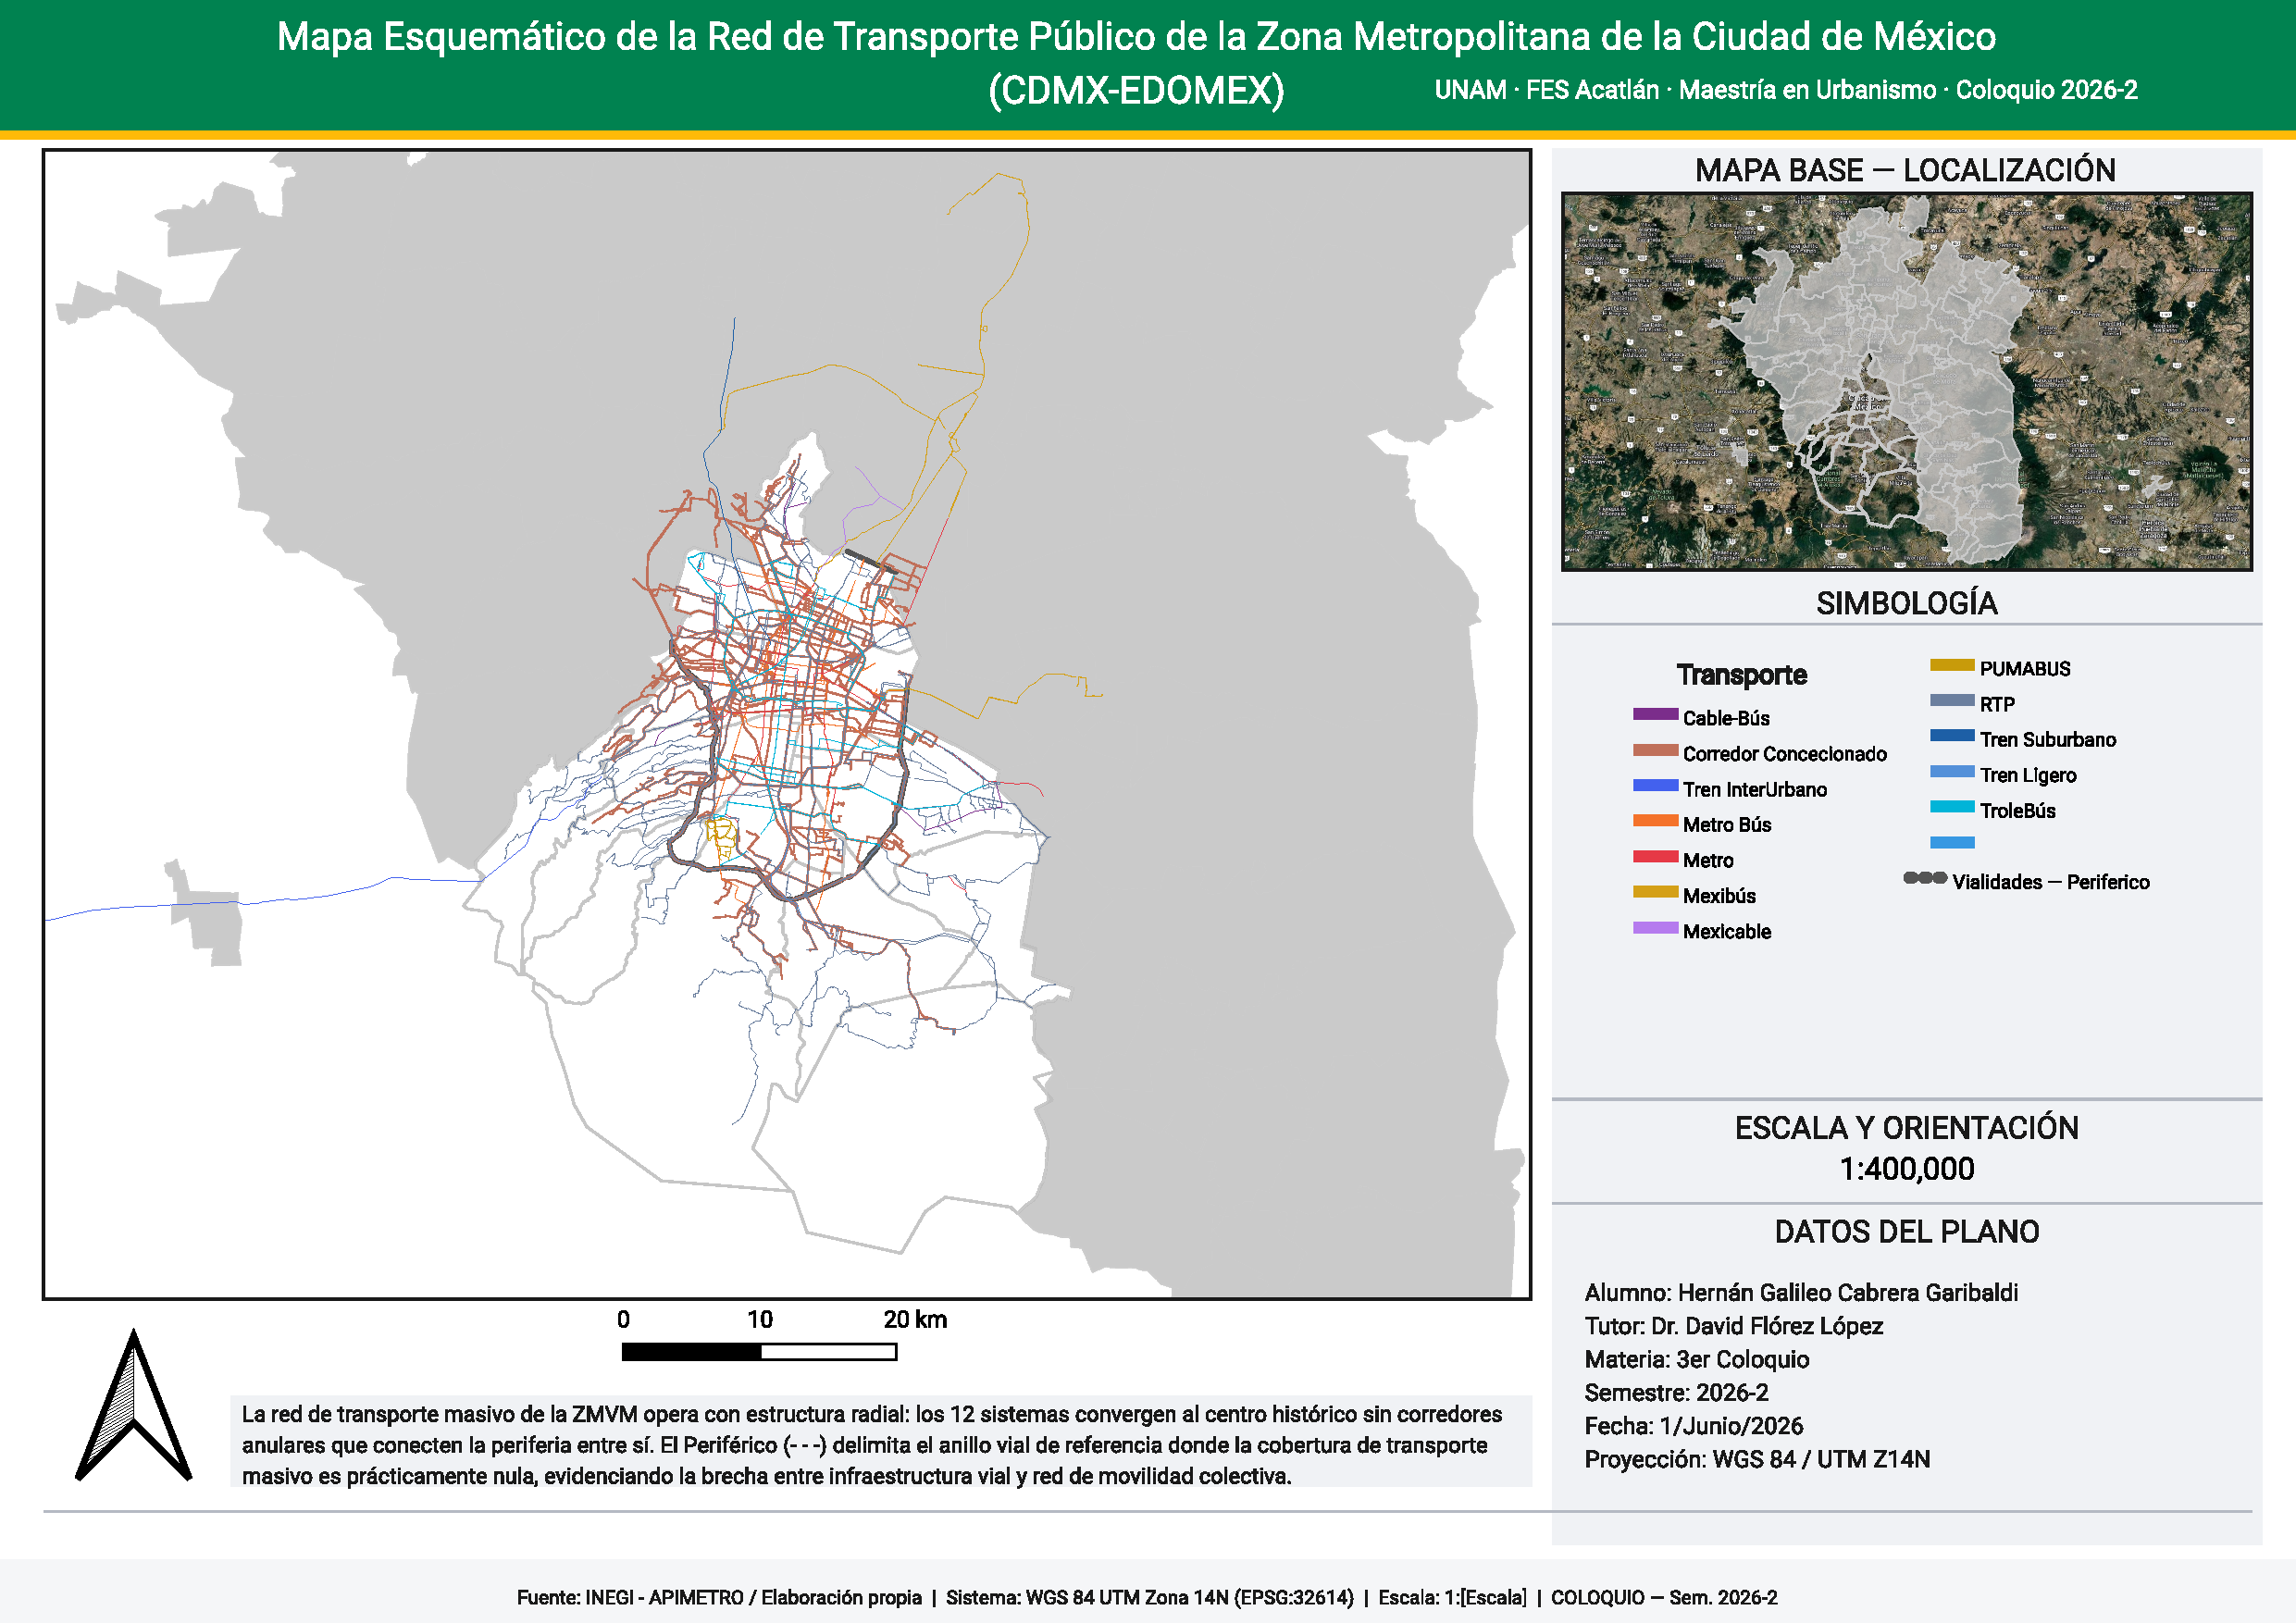
\includegraphics[width=\textwidth]{Figures/Mapas/Mapa_Red_Esquematica}
  \caption[Red esquemática multimodal de la ZMVM (alta resolución)]{Red esquemática multimodal de la \zmvm{}.
    Muestra los doce sistemas de transporte reconocidos por el modelo VFT sobre los límites político-administrativos
    de la \cdmx{} y el Estado de México.
    \fuentefigura{Elaboración propia con \textbf{Transport-gis-zmvm-mjg};
    datos: \textsc{gtfs} \textsc{semovi} 2024 e \textsc{inegi} 2023.}}
  \label{fig:anx-mapa-red}
\end{figure}

% =============================================================================
\section{Cobertura Espacial — Isócronas 800~m}
\label{anx:mapa-cobertura-total}
% =============================================================================

\begin{figure}[p]
  \centering
  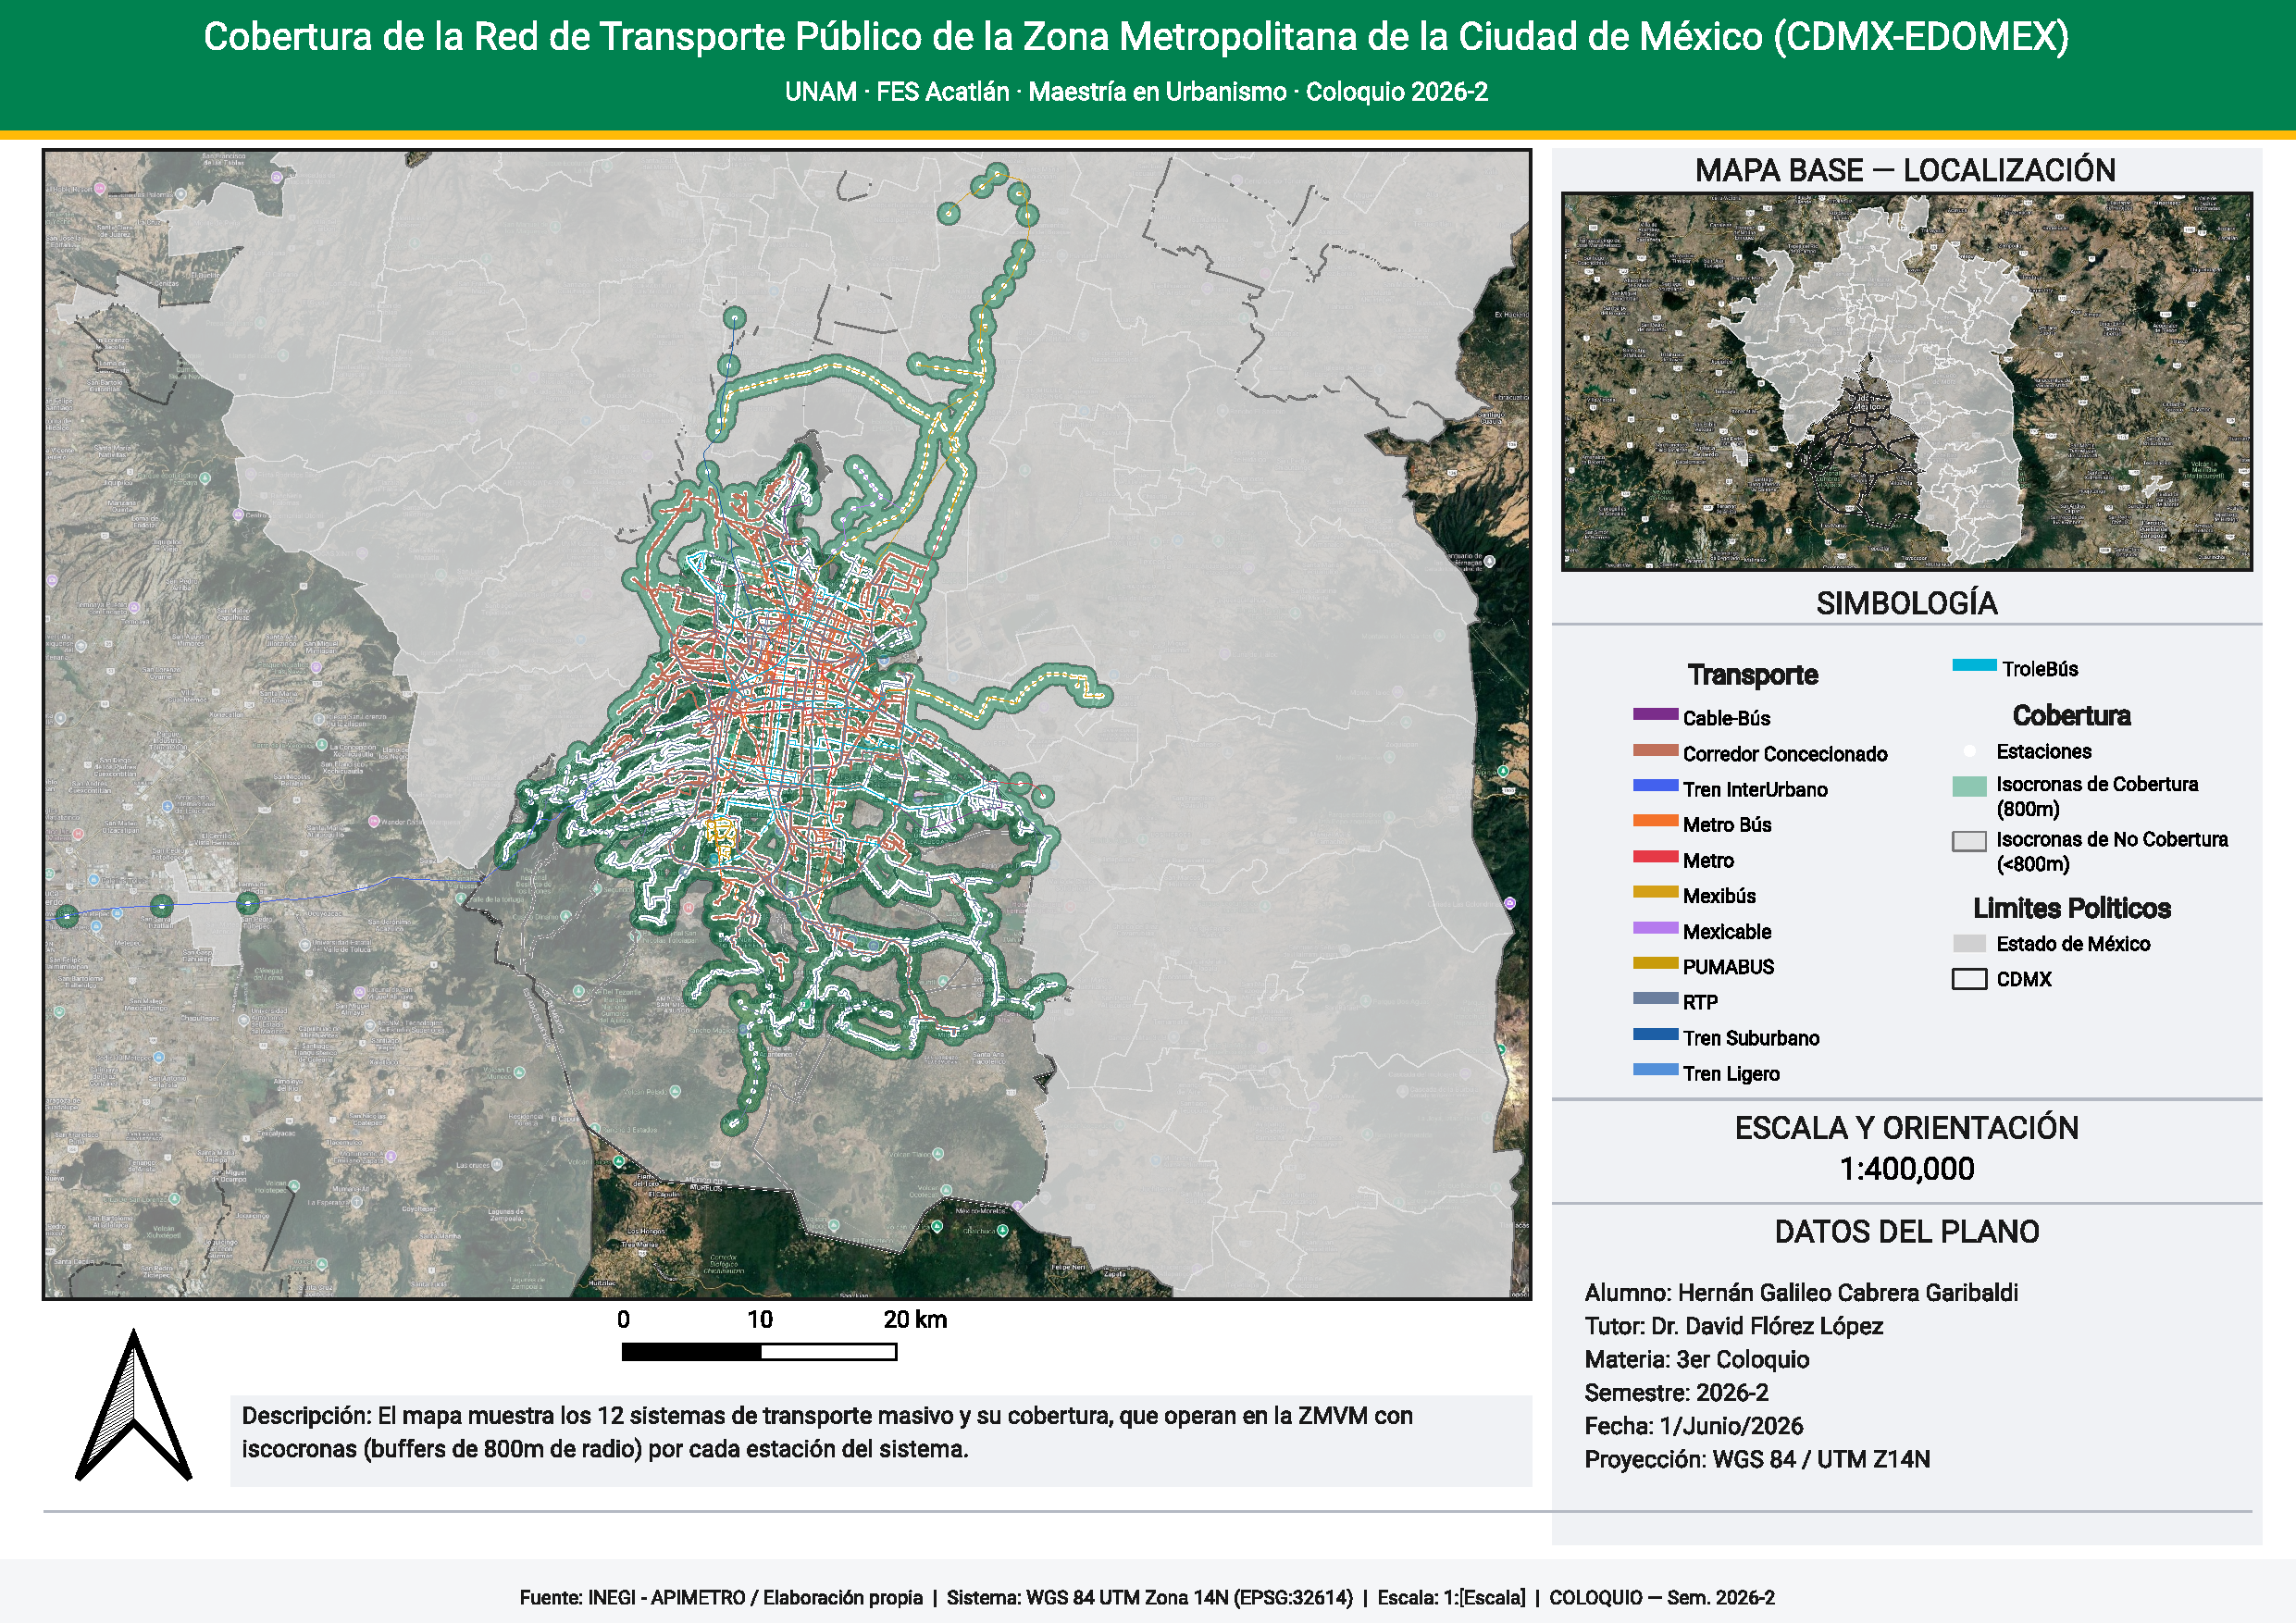
\includegraphics[width=\textwidth]{Figures/Mapas/Mapa_Cobertura_Red_Total}
  \caption[Cobertura de la red por isócronas de 800~m (alta resolución)]{Cobertura espacial de la red multimodal de transporte
    de la \zmvm{}, calculada como el área alcanzable a 800~m de caminata desde cualquier parada o estación
    (indicador $C$ del modelo VFT). Las alcaldías del sur presentan las coberturas más bajas.
    \fuentefigura{Elaboración propia con \textbf{Transport-gis-zmvm-mjg};
    datos: \textsc{gtfs} \textsc{semovi} 2024 e \textsc{inegi} 2023.}}
  \label{fig:anx-mapa-cobertura-total}
\end{figure}

% =============================================================================
\section{Cobertura Espacial — Mapa de Calor}
\label{anx:mapa-cobertura-calor}
% =============================================================================

\begin{figure}[p]
  \centering
  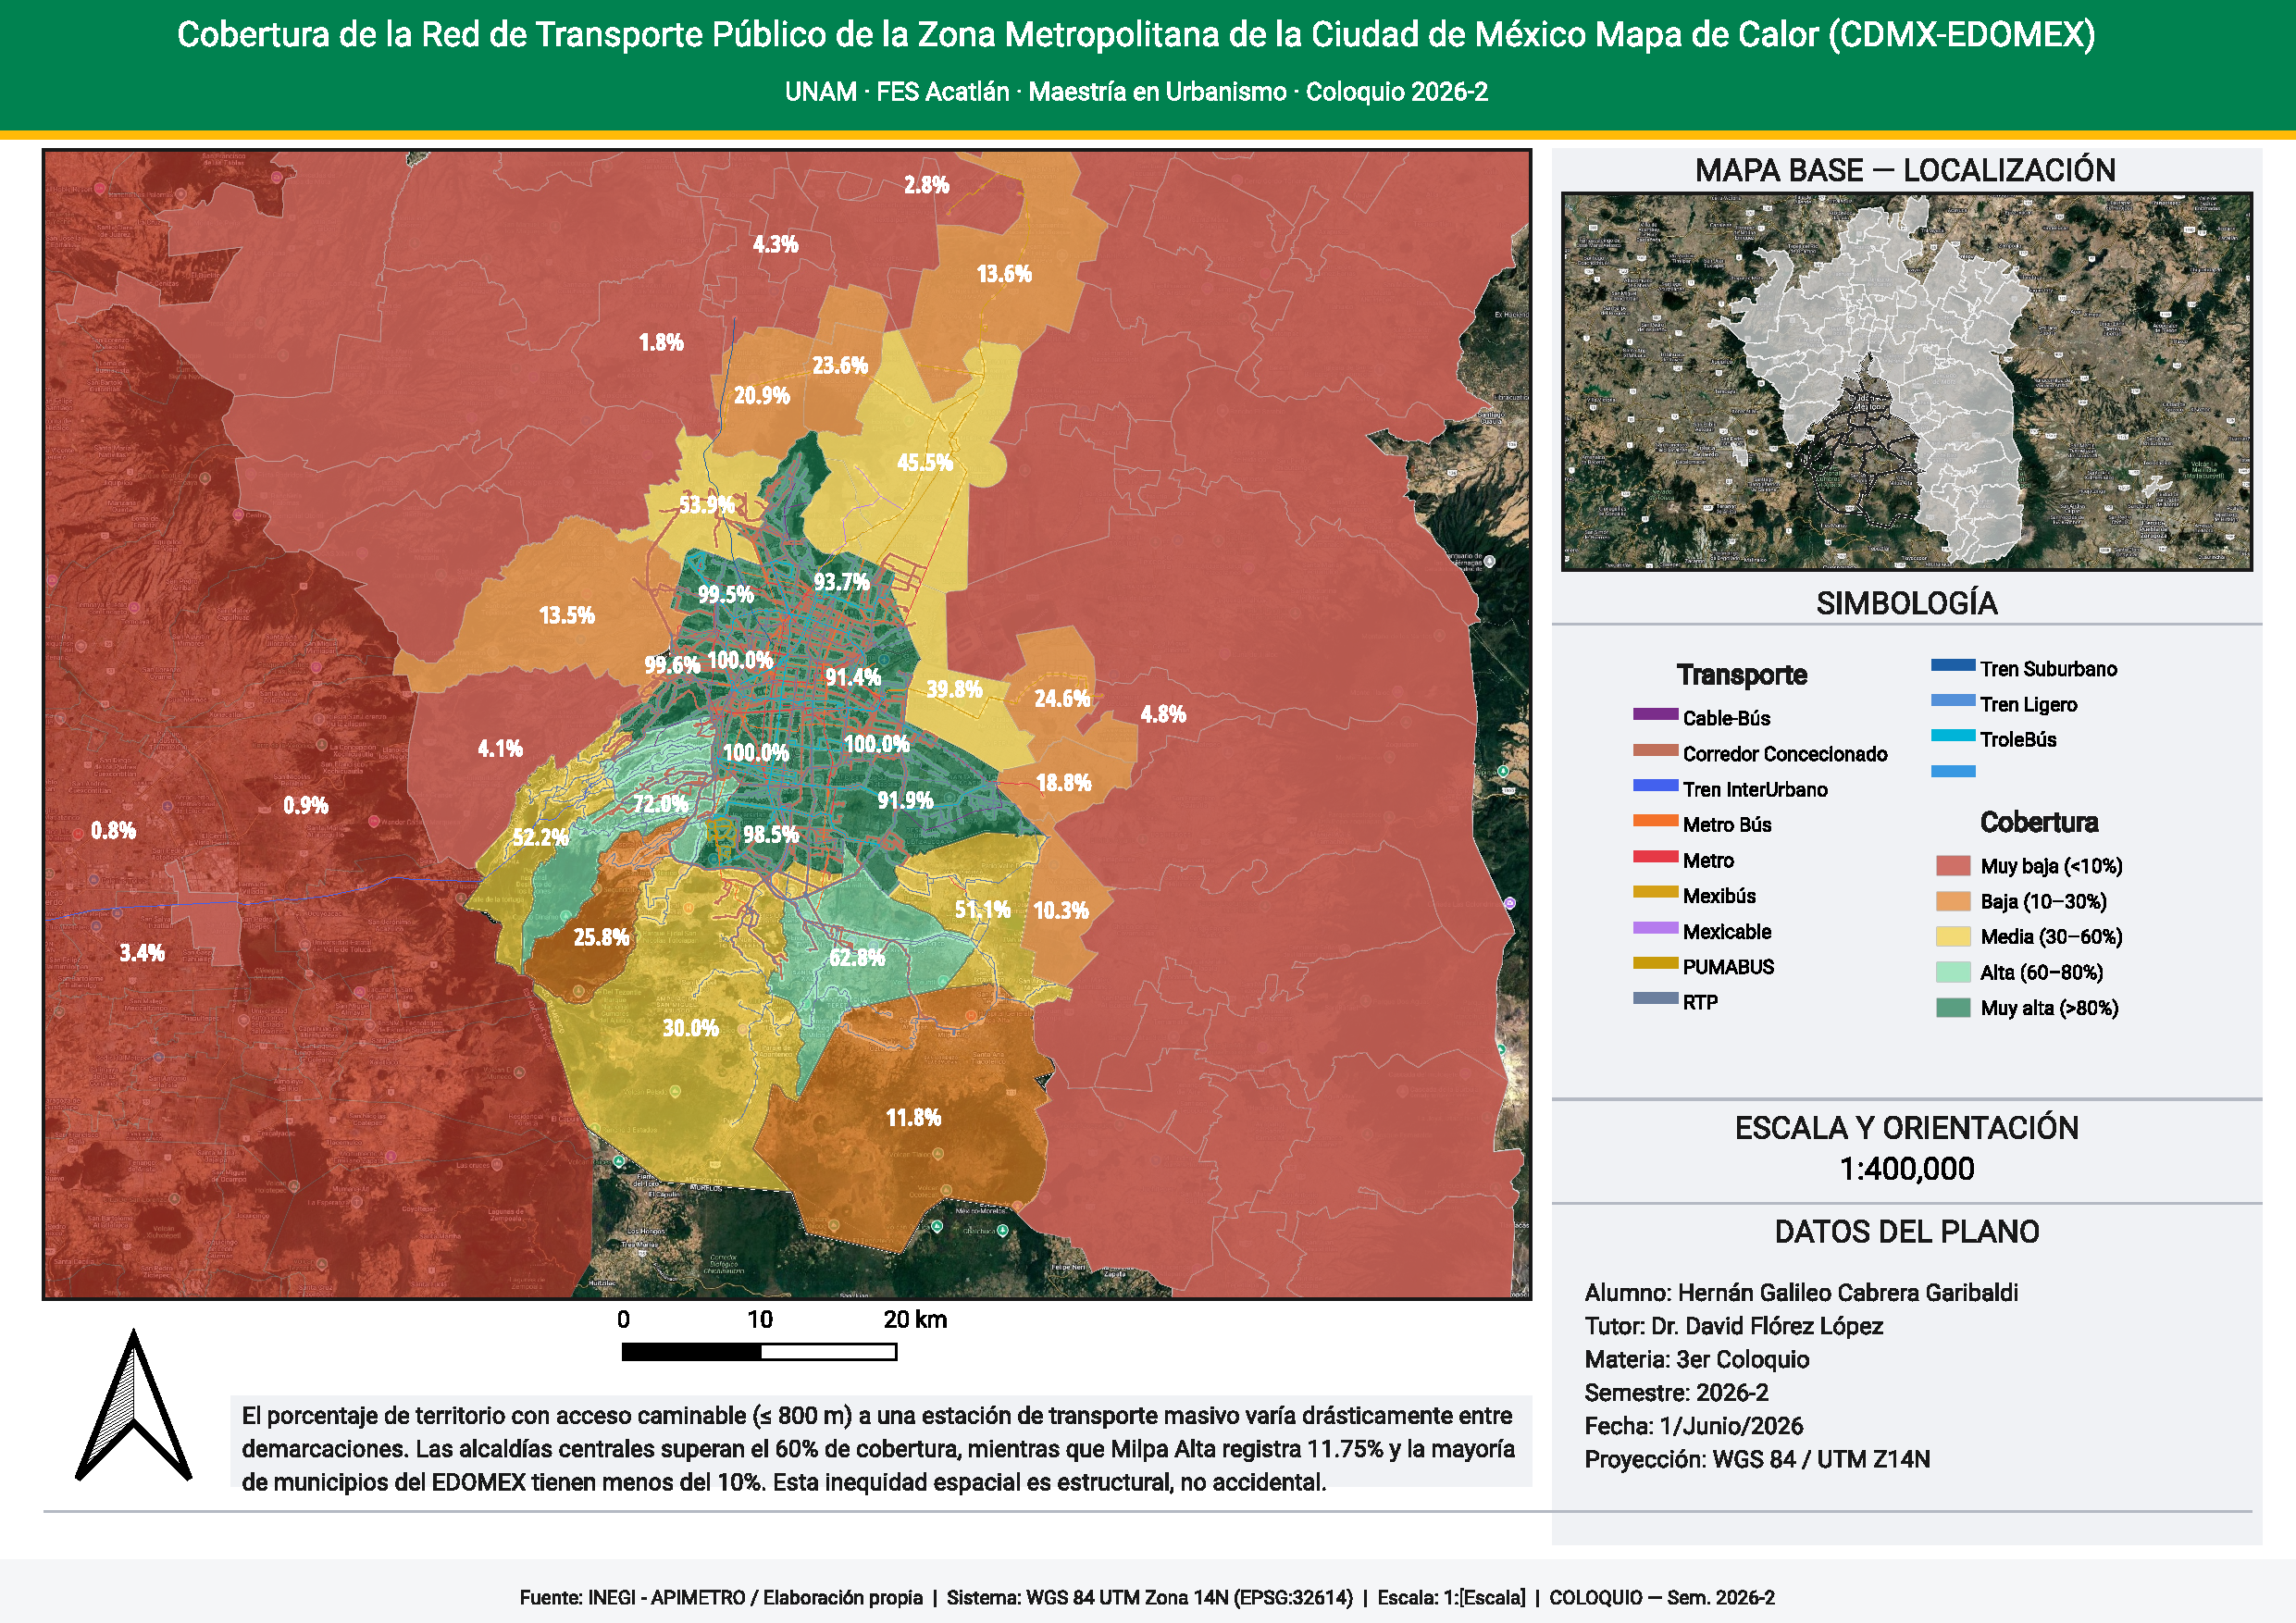
\includegraphics[width=\textwidth]{Figures/Mapas/Mapa_Cobertura_Mapa_Calor}
  \caption[Densidad de cobertura — mapa de calor (alta resolución)]{Densidad de la cobertura espacial de la red
    representada como mapa de calor. La intensidad del color refleja la concentración de isócronas superpuestas,
    revelando los núcleos de mayor accesibilidad modal en la región metropolitana.
    \fuentefigura{Elaboración propia con \textbf{Transport-gis-zmvm-mjg};
    datos: \textsc{gtfs} \textsc{semovi} 2024 e \textsc{inegi} 2023.}}
  \label{fig:anx-mapa-cobertura-calor}
\end{figure}

% =============================================================================
\section{Fuerza Capilar — Nodos \textit{Hub} Principales}
\label{anx:mapa-fuerza-capilar}
% =============================================================================

\begin{figure}[p]
  \centering
  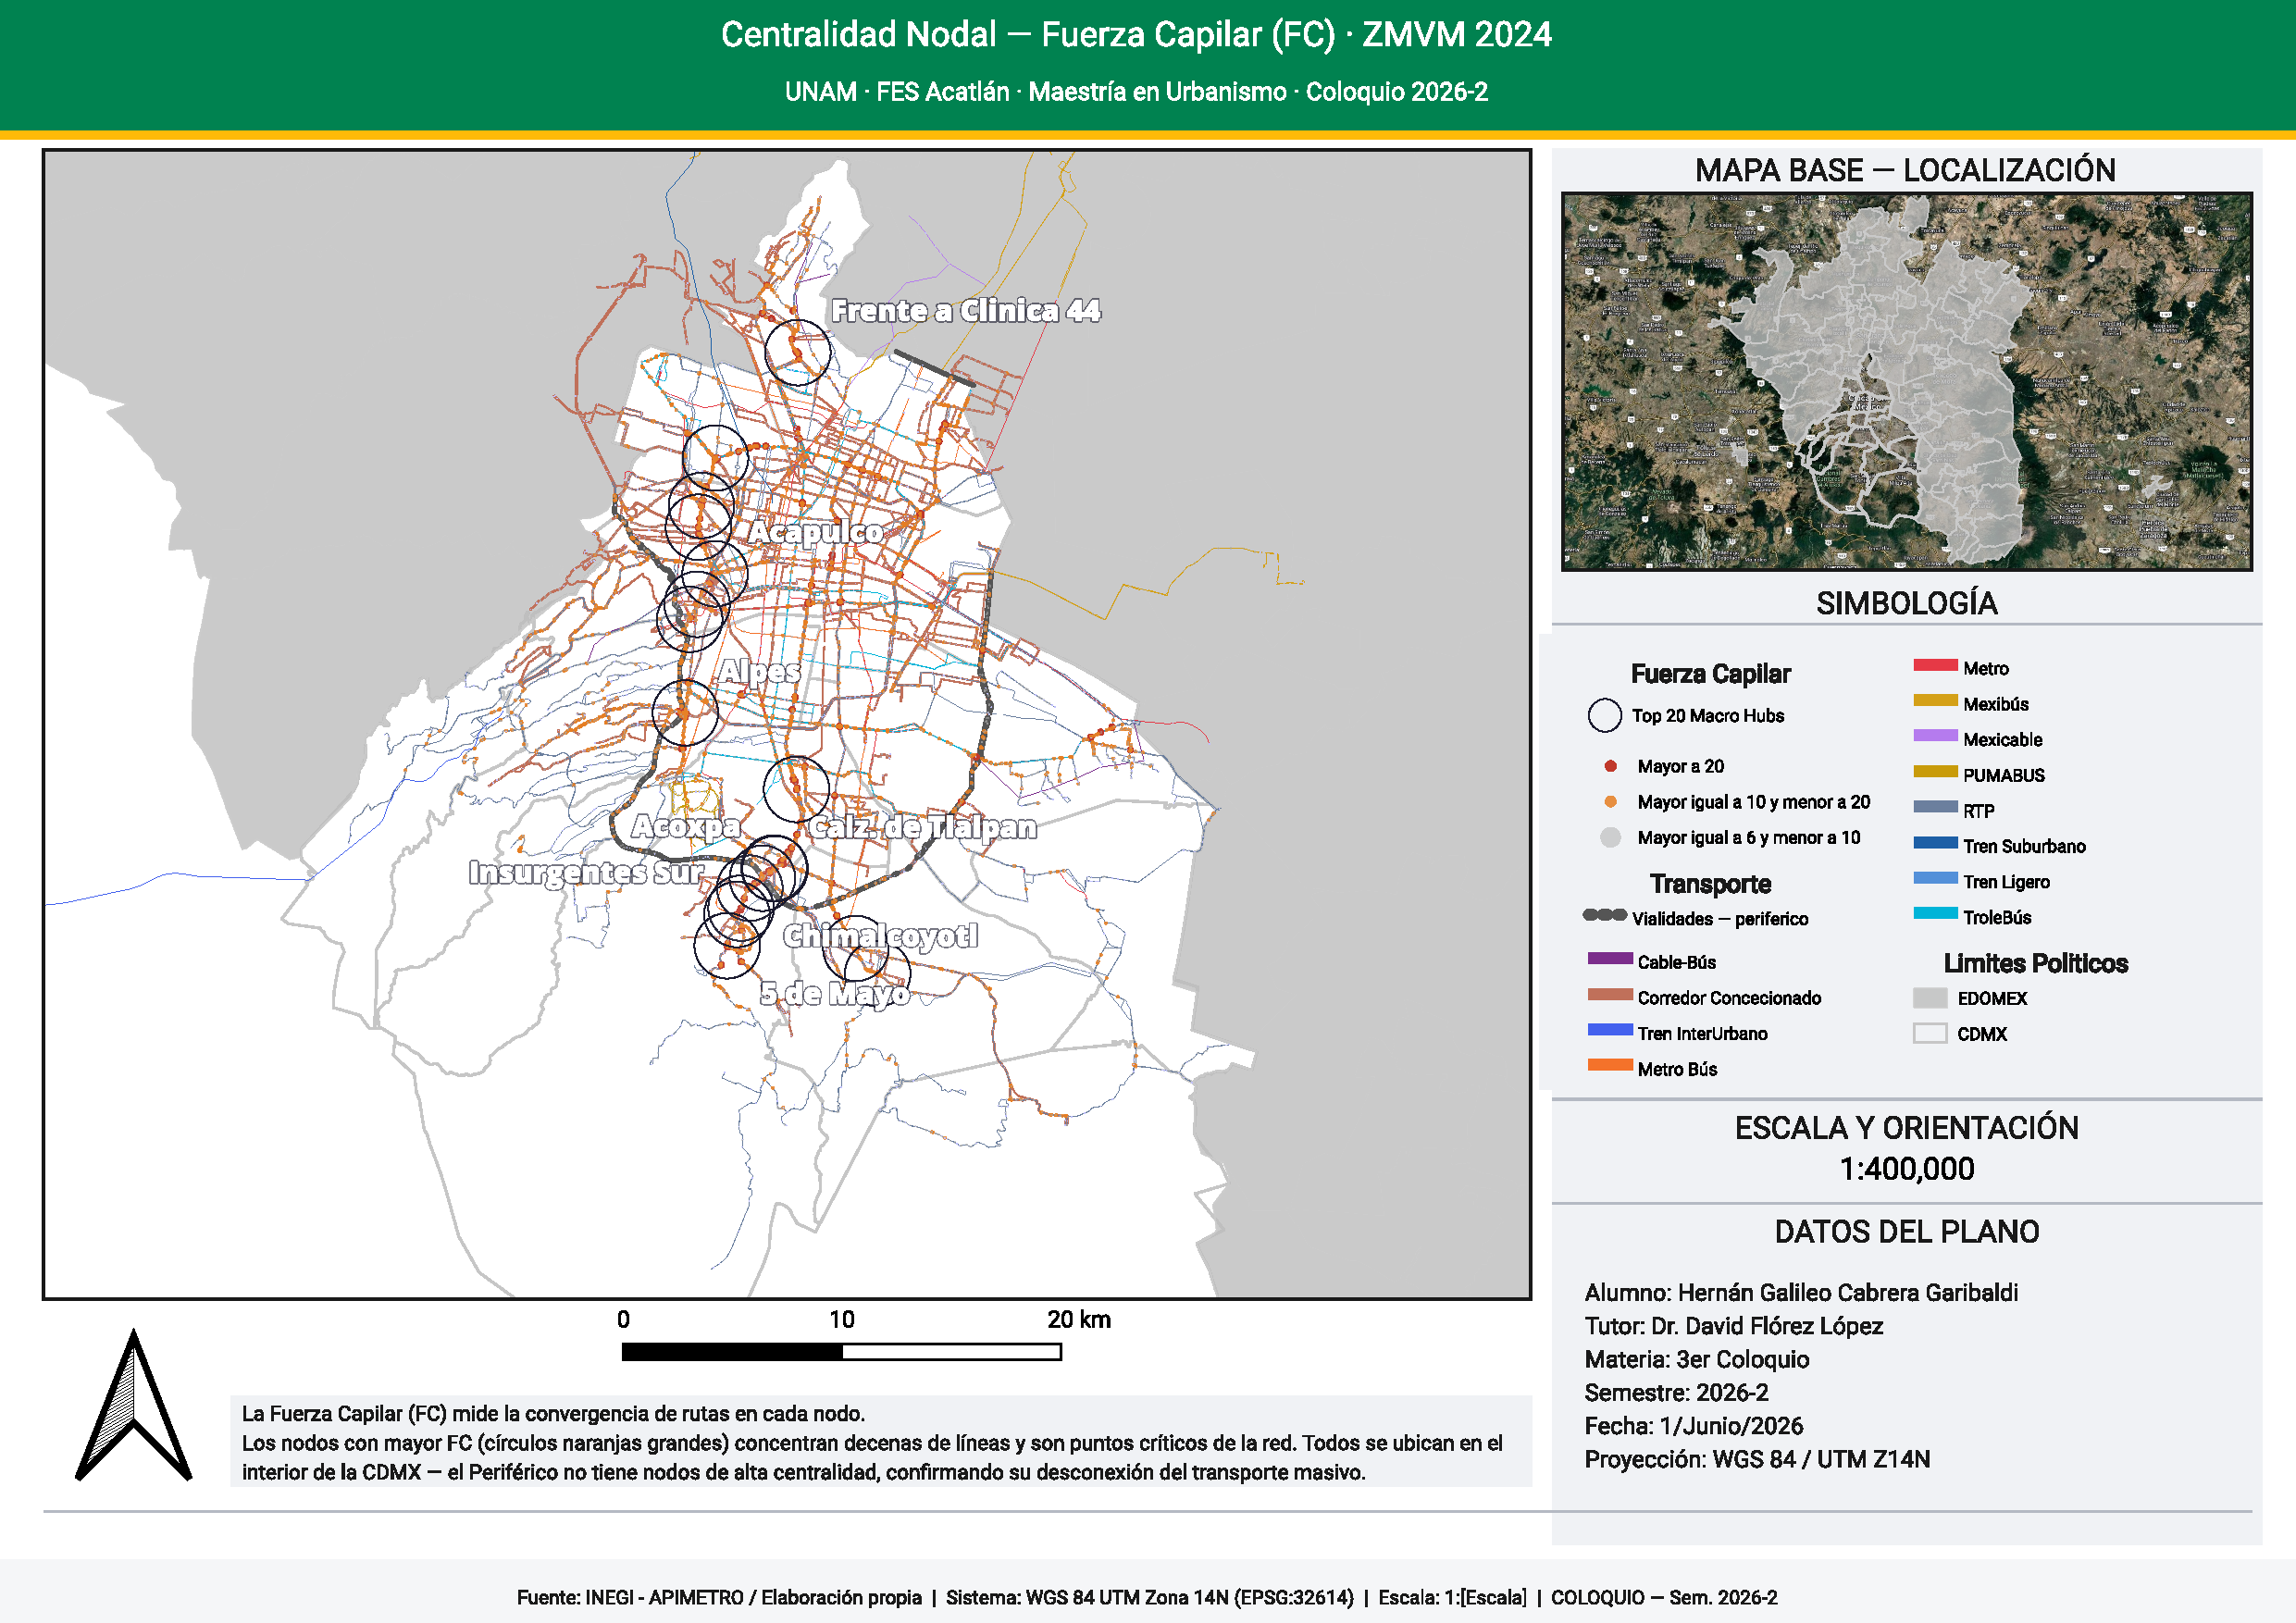
\includegraphics[width=\textwidth]{Figures/Mapas/Mapa_Fuerza_Capilar}
  \caption[Fuerza capilar: los 20 nodos \textit{hub} de mayor centralidad (alta resolución)]{Fuerza capilar de los nodos de la red
    de transporte de la \zmvm{}. Se destacan los 20 nodos con mayor valor de centralidad de intermediación ponderada,
    que corresponden a los puntos de mayor influencia redistributiva de flujos en la red multimodal.
    \fuentefigura{Elaboración propia con \textbf{Transport-gis-zmvm-mjg};
    datos: \textsc{gtfs} \textsc{semovi} 2024 e \textsc{inegi} 2023.}}
  \label{fig:anx-mapa-fuerza-capilar}
\end{figure}

% =============================================================================
\section{Factor de Desviación por Nodo}
\label{anx:mapa-factor-desviacion}
% =============================================================================

\begin{figure}[p]
  \centering
  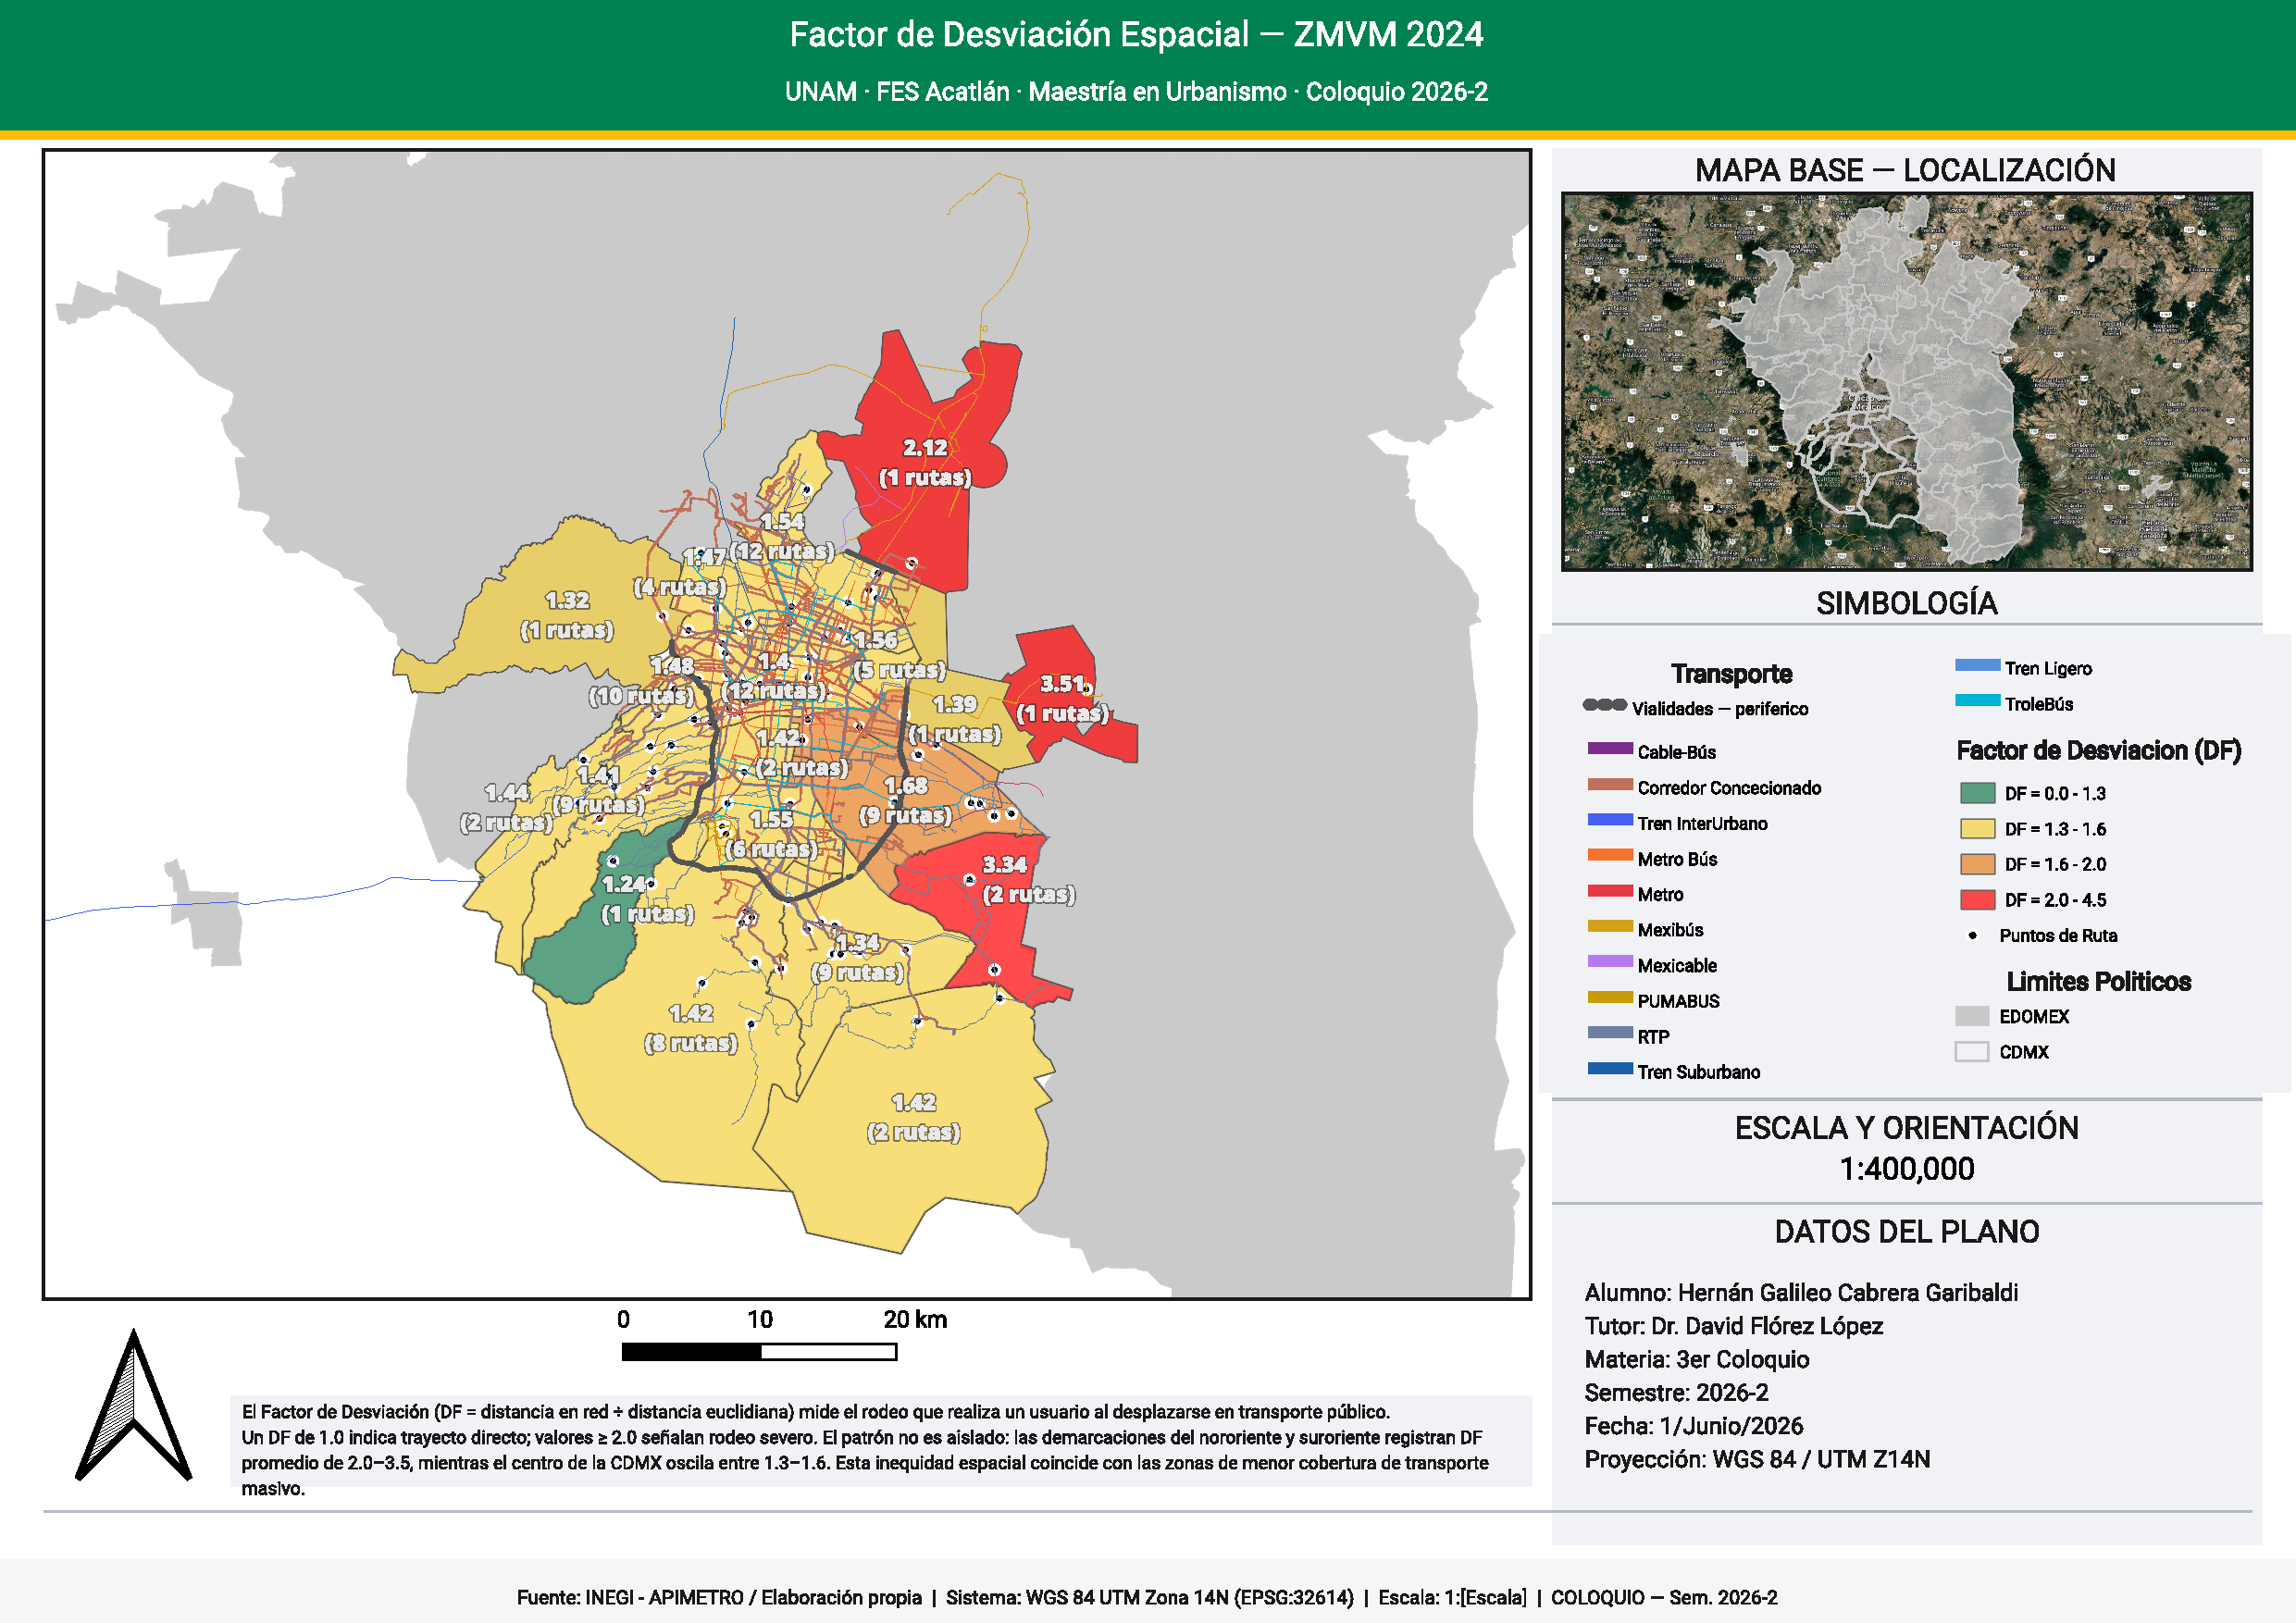
\includegraphics[width=\textwidth]{Figures/Mapas/Mapa_DF}
  \caption[Factor de desviación por nodo (alta resolución)]{Factor de desviación ($\text{FD}$) de los nodos de la red
    de transporte de la \zmvm{}. El gradiente de color (verde→rojo) indica la relación entre la distancia real de viaje
    y la distancia euclidiana óptima: valores altos (rojo) señalan nodos donde las rutas disponibles desvían significativamente
    del trayecto directo, lo que penaliza la eficiencia de la red en esas zonas.
    \fuentefigura{Elaboración propia con \textbf{Transport-gis-zmvm-mjg};
    datos: \textsc{gtfs} \textsc{semovi} 2024 e \textsc{inegi} 2023.}}
  \label{fig:anx-mapa-factor-desviacion}
\end{figure}
